%%%%%%%%%%%%%%%%%%%%%%%%%%% asme2ej.tex %%%%%%%%%%%%%%%%%%%%%%%%%%%%%%%
% Template for producing ASME-format journal articles using LaTeX    %
% Written by   Harry H. Cheng, Professor and Director                %
%              Integration Engineering Laboratory                    %
%              Department of Mechanical and Aeronautical Engineering %
%              University of California                              %
%              Davis, CA 95616                                       %
%              Tel: (530) 752-5020 (office)                          %
%                   (530) 752-1028 (lab)                             %
%              Fax: (530) 752-4158                                   %
%              Email: hhcheng@ucdavis.edu                            %
%              WWW:   http://iel.ucdavis.edu/people/cheng.html       %
%              May 7, 1994                                           %
% Modified: February 16, 2001 by Harry H. Cheng                      %
% Modified: January  01, 2003 by Geoffrey R. Shiflett                %
% Use at your own risk, send complaints to /dev/null                 %
%%%%%%%%%%%%%%%%%%%%%%%%%%%%%%%%%%%%%%%%%%%%%%%%%%%%%%%%%%%%%%%%%%%%%%

% Hoch 3 beispielbilder
% hoch 1, schräg 2 weitere



%%% use twocolumn and 10pt options with the asme2ej format
\documentclass[twocolumn,10pt]{asme2ej}

\usepackage{graphicx} %% for loading jpg figures
\usepackage{hyperref}   % to set up hyperlinks
\hypersetup{
	colorlinks=true,
	linkcolor=blue,
	citecolor=blue,
	urlcolor=blue,
}
\usepackage[square,numbers]{natbib}
\usepackage{float}
\usepackage{tikz}
\usepackage{amsmath}
\usepackage{listings}

\newcommand*\redcircled[1]{\tikz[baseline=(char.base)]{
            \node[shape=circle,draw,inner sep=2pt, fill=red!40] (char) {#1};}}
\newcommand*\bluecircled[1]{\tikz[baseline=(char.base)]{
            \node[shape=circle,draw,inner sep=2pt, fill=blue!40] (char) {#1};}}

            \usepackage{xcolor}

            \definecolor{codegreen}{rgb}{0,0.6,0}
            \definecolor{codegray}{rgb}{0.5,0.5,0.5}
            \definecolor{codepurple}{rgb}{0.58,0,0.82}
            \definecolor{backcolour}{rgb}{0.95,0.95,0.92}
            
            \lstdefinestyle{mystyle}{
                backgroundcolor=\color{backcolour},   
                commentstyle=\color{codegreen},
                keywordstyle=\color{magenta},
                numberstyle=\tiny\color{codegray},
                stringstyle=\color{codepurple},
                basicstyle=\ttfamily\footnotesize,
                breakatwhitespace=false,         
                breaklines=true,                 
                captionpos=b,                    
                keepspaces=true,                 
                numbers=left,                    
                numbersep=5pt,                  
                showspaces=false,                
                showstringspaces=false,
                showtabs=false,                  
                tabsize=2
            }
            
\lstset{style=mystyle}

% \usepackage{url}
% \usepackage{breakurl}
% \usepackage[breaklinks]{hyperref}   
%\def\UrlBreaks{\do\/\do-}

%% The class has several options
%  onecolumn/twocolumn - format for one or two columns per page
%  10pt/11pt/12pt - use 10, 11, or 12 point font
%  oneside/twoside - format for oneside/twosided printing
%  final/draft - format for final/draft copy
%  cleanfoot - take out copyright info in footer leave page number
%  cleanhead - take out the conference banner on the title page
%  titlepage/notitlepage - put in titlepage or leave out titlepage
%  
%% The default is oneside, onecolumn, 10pt, final


\title{Computer Vision SS22 Assignment 2: Camera Calibration}

%%% first author
\author{Felix Hamburger
    \affiliation{
	Student ID: 35925\\
	Computer Vision SS22\\
	Computer Science Master\\
	Ravensburg Weingarten University\\
    Email: felix.hamburger@rwu.de
    }	
}

%%% second author
%%% remove the following entry for single author papers
%%% add more entries for additional authors
\author{Mario Amann
    \affiliation{ 
    Student ID: 35926\\
    Computer Vision SS22\\
    Computer Science Master\\
    Ravensburg Weingarten University\\
    Email: mario.amann@rwu.de
     }	
}



\begin{document}

\maketitle   

% Notes:
% Citations
% https://answers.opencv.org/question/32411/opencv-bibtex-citation/
% http://citebay.com/how-to-cite/opencv/

% Functions:

% imread: https://docs.opencv.org/3.4/d4/da8/group__imgcodecs.html#ga288b8b3da0892bd651fce07b3bbd3a56

% cvtColor: https://docs.opencv.org/3.4/de/d25/imgproc_color_conversions.html
% RGB[A] to Gray:Y←0.299⋅R+0.587⋅G+0.114⋅B


%%%%%%%%%%%%%%%%%%%%%%%%%%%%%%%%%%%%%%%%%%%%%%%%%%%%%%%%%%%%%%%%%%%%%%
\begin{abstract}
{\it This paper shows in four steps how a pinhole camera model with radial distortion can be undistorted.
It shows how the intrinsic and extrinsic properties of the camera can be used to undo the distortion for images taken with this camera.
}
\end{abstract}

%%%%%%%%%%%%%%%%%%%%%%%%%%%%%%%%%%%%%%%%%%%%%%%%%%%%%%%%%%%%%%%%%%%%%%
%\begin{nomenclature}
% \entry{A}{You may include nomenclature here.}
%\entry{$\alpha$}{There are two arguments for each entry of the nomemclature environment, the symbol and the definition.}
% \end{nomenclature}

%The primary text heading is  boldface and flushed left with the left margin.  The spacing between the  text and the heading is two line spaces.

%%%%%%%%%%%%%%%%%%%%%%%%%%%%%%%%%%%%%%%%%%%%%%%%%%%%%%%%%%%%%%%%%%%%%%
\section{Introduction}
\label{section:introduction}
\noindent
\begin{figure}[H]
    \centerline{\includegraphics[width=2.5in]{output/curvy_lines.PNG}}
    \caption{Depiction of the undistorted image with lines indicating wrongt dimensions of the chess board.}
    \label{fig:curvylines}
\end{figure}


%%%%%%%%%%%%%%%%%%%%%%%%%%%%%%%%%%%%%%%%%%%%%%%%%%%%%%%%%%%%%%%%%%%%%%
\section{Preprocessing}
\label{section:preprocessing}
\noindent
Before any preprocessing can be applied, the images have to be created from the given video. Therefore each frame of the video is saved separately. This is done with the imread function\cite{opencv_imread} of OpenCV which 
outputs the image as numpy array with the shape (Height, Width, Channel). By default the decoded image is stored in the BGR-format. Which means, the first channel contains the
blue color channel, the second one contains the green color channel and the last the red one. In preparation for the detection of the checkerboard pattern, the images are converted to grayscale format. 
This convertion is made with the cvtColor function\cite{opencv_cvtColor} of OpenCV. The convertion of colorspace is made with the following
formula\cite{opencv_rgb2gray}:
\begin{center}
    $Y = B * 0.114 + G * 0.587 + R * 0.299$
    \label{eq_rgb2gray}
\end{center}



%findChessboardCorners: https://docs.opencv.org/4.x/d9/d0c/group__calib3d.html#ga93efa9b0aa890de240ca32b11253dd4a

%%%%%%%%%%%%%%%%%%%%%%%%%%%%%%%%%%%%%%%%%%%%%%%%%%%%%%%%%%%%%%%%%%%%%%
\section{Corner Detection}
\label{section:cornerdetection}

\noindent
After the preprocessing steps, the corners of the chessboard can be detected on the images. For this the OpenCV function findChessboardCorners\cite{opencv_findChessboardCorners} is used. As input parameters the function gets a grayscale image, the size of the pattern and already recognized corners. As size of the pattern the size 6 times 6 was chosen, because in about 500 pictures from 2000 the chessboard is recognized and the chessboard is recognized at completely different places. Since no corners are recognized before, nothing is passed at the already recognized corners. Furthermore, no flag is used and needed because the images were already converted to grayscale in preprocessing, incorrectly extracted squares were manually checked and did not occur, and there was no time pressure to speed up the detection of the corners.
If corners of a chessboard are found in the image, the corner points are added to a list of corner points from all images.
%%%%%%%%%%%%%%%%%%%%%%%%%%%%%%%%%%%%%%%%%%%%%%%%%%%%%%%%%%%%%%%%%%%%%
\section{Camera Calibration}
\label{section:calibration}
\noindent

With the list of corner points the intrinsic camera parameters can be estimated. 
The OpenCV function calibrateCamera\cite{opencv_calibrateCamera} is used, which is based on the algorithm of the paper by Z.Zhang\cite{zhang2000flexible} from 2000. 
The first parameter passed is a matrix consisting of vectors of the calibration points in the coordinate space. In this case this matrix is a multi-dimensional meshgrid. Furthermore the list of corner points from the \nameref{section:edgedetection} section and the size of the image are passed to the function. The remaining passing parameters are passed as NoneType and no flags are set. The function returns the root mean squared re-projection error, the intrinsic camera matrix, the distortion coefficients and the rotation and translation vectors.
The intrinsic camera matrix is described as follows: 
\begin{center}
    $K = \begin{bmatrix}
   f_x & 0 & c_x \\
   0 & f_y & c_y \\
   0 & 0 & 1
   \end{bmatrix}
   $
    \label{eq_intrinsicmatrix}
\end{center}
The returned intrinsic camera matrix from the calibrateCamera function has the values:
@@@@@@@@@@@@@@@@@@@@
\begin{center}
    $K = \begin{bmatrix}
   f_x & 0 & c_x \\
   0 & f_y & c_y \\
   0 & 0 & 1
   \end{bmatrix}
   $
    \label{eq_calculatedintrinsicmatrix}
\end{center}
The calibrateCamera function returns following distortion coefficients:
@@@@@@@@@@@@@@@@@@@@
\begin{center}
    $k_1 = s$\\
    $k_2 = s$\\
    $p_1 = s$\\
    $p_2 = s$\\
    $k_1 = s$\\
    $k_1 = s$
    \label{eq_distcoeff}
\end{center}
As next step the optimal camera intrinsic matrix has to be computed. For this purpose the getOptimalNewCameraMatrix function\cite{opencv_getOptimalNewCameraMatrix} is used. The function computes the optimal camera intrinsic matrix based on free scaling parameter alpha.
The camera matrix, the distortion coefficients vector, the original and the new image size and the free scaling parameter alpha are passed as input. No further optional parameter are passed. The camera matrix and the distortion coefficients vector are the previously calculated values. As original and new image size the original size of the image is passed. The free scaling parameter alpha is set to one. Therefore all pixels are kept and no pixels are removed \cite{opencv_calibrationtutorial}.
The optimal intrinsic camera matrix from getOptimalNewCameraMatrix has the following values:
@@@@@@@@@@@@@@@@@@@@
\begin{center}
    $K = \begin{bmatrix}
   f_x & 0 & c_x \\
   0 & f_y & c_y \\
   0 & 0 & 1
   \end{bmatrix}
   $
    \label{eq_optintrinsicmatrix}
\end{center}
With the optimal intrinsic matrix the next step the undistortion can take place.

\section{Undistortion}
\label{section:undistortion}
\noindent

\begin{figure}[H]
    \centerline{\includegraphics[width=2.5in]{output/straight_lines.PNG}}
    \caption{Depiction of the undistorted image with lines indicating the correct dimensions of the chess board.}
    \label{fig:straightlines}
\end{figure}

\section{Summary}
\label{section:summary}

\begin{figure}[H]
\centerline{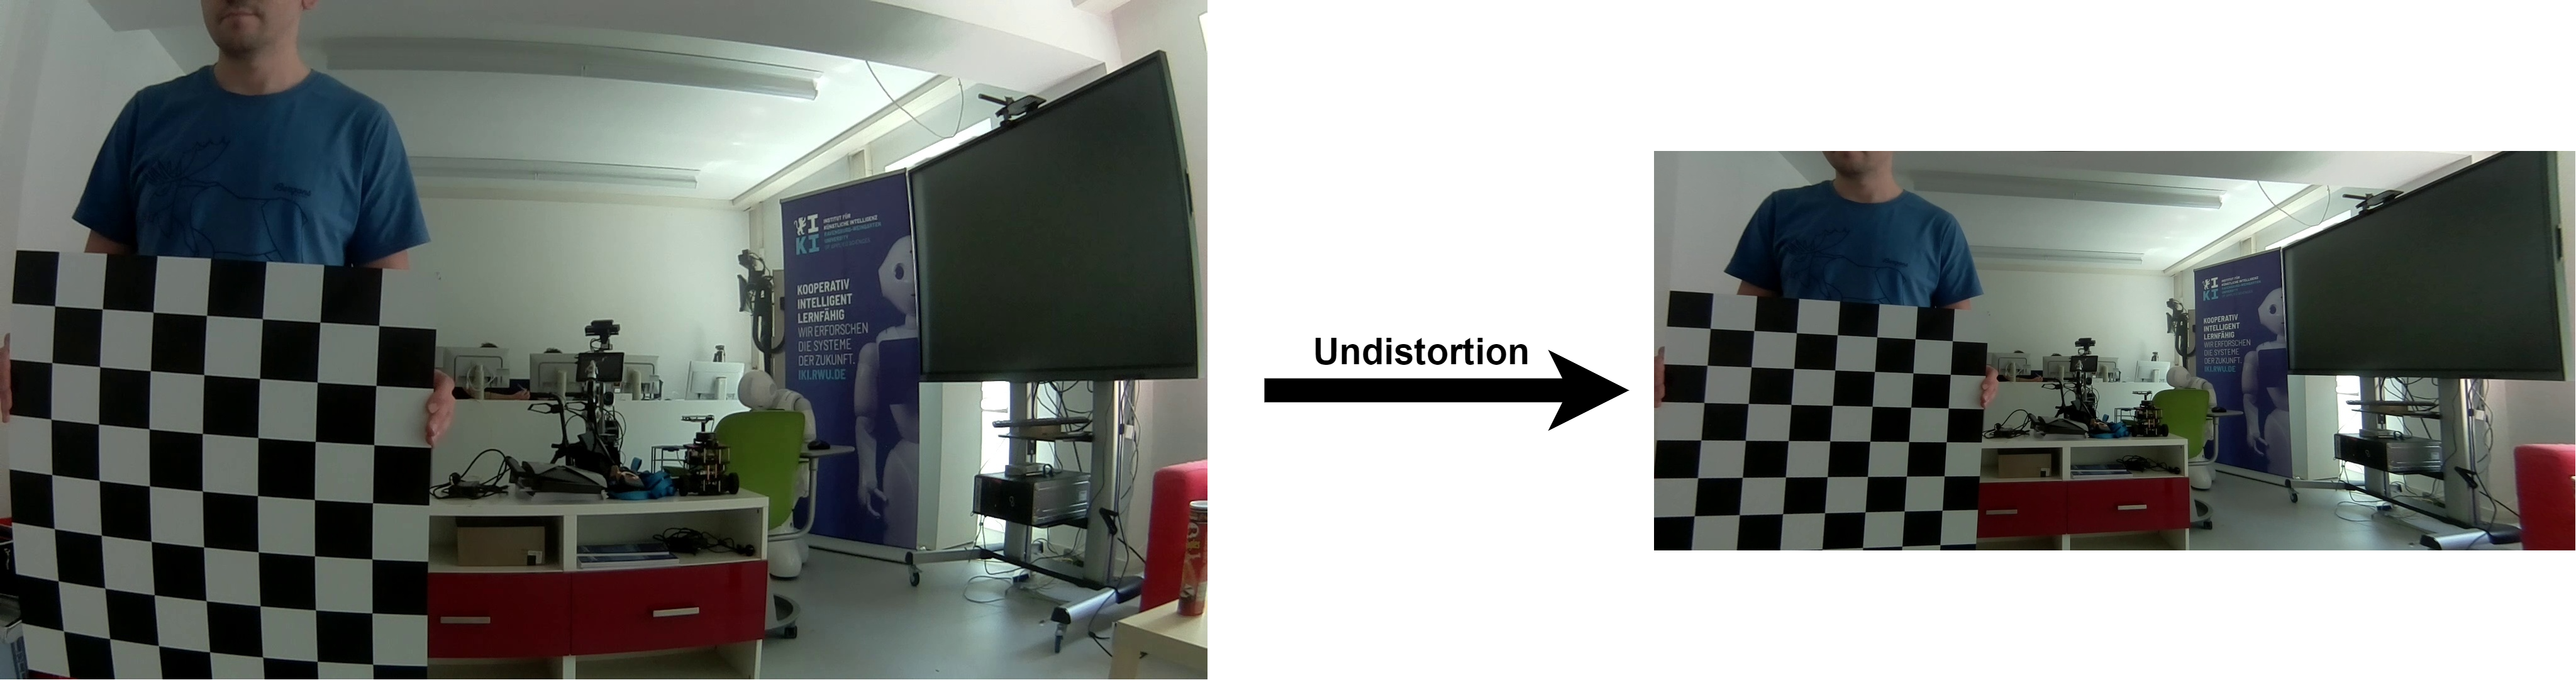
\includegraphics[width=2.5in]{output/res1.png}}
\caption{Depiction of the final undistortion with the chess board located in the bottom left corner.}
\label{fig:res1}
\end{figure}

\begin{figure}[H]
    \centerline{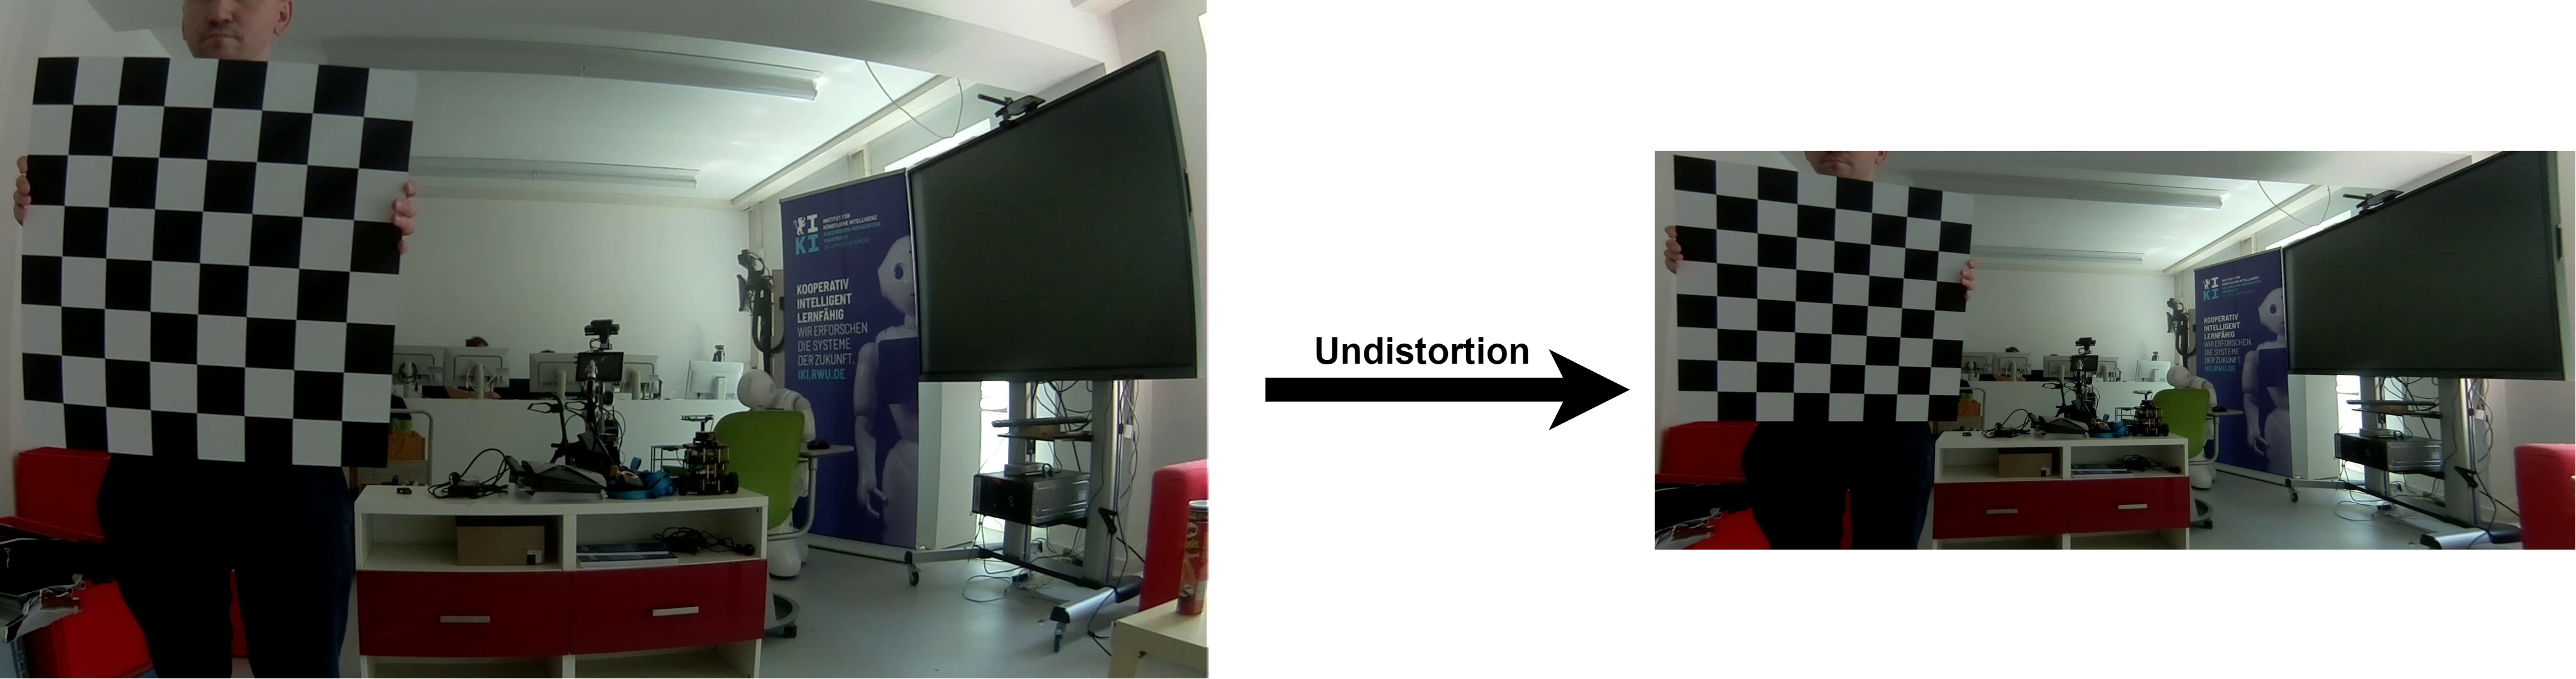
\includegraphics[width=2.5in]{output/res2.png}}
    \caption{Depiction of the final undistortion with the chess board located in the upper left corner.}
    \label{fig:res2}
\end{figure}

\begin{figure}[H]
    \centerline{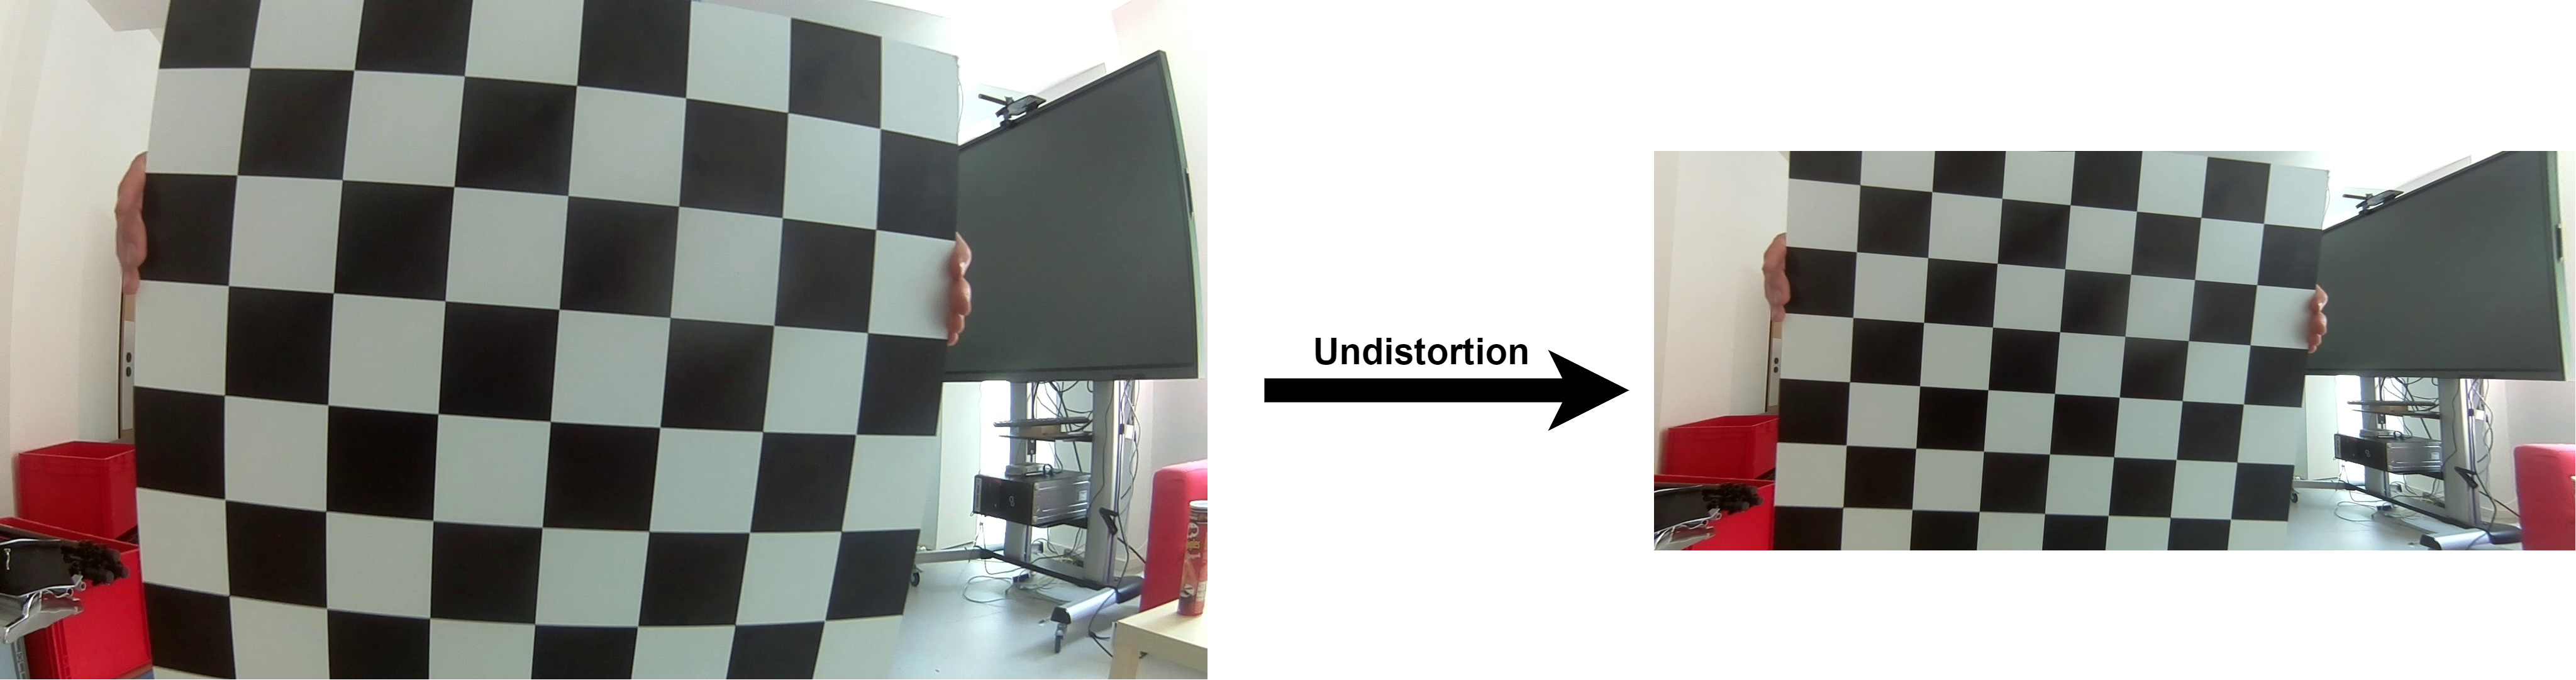
\includegraphics[width=2.5in]{output/res3.png}}
    \caption{Depiction of the final undistortion with the chess board located in the center.}
    \label{fig:res3}
\end{figure}

\begin{figure}[H]
    \centerline{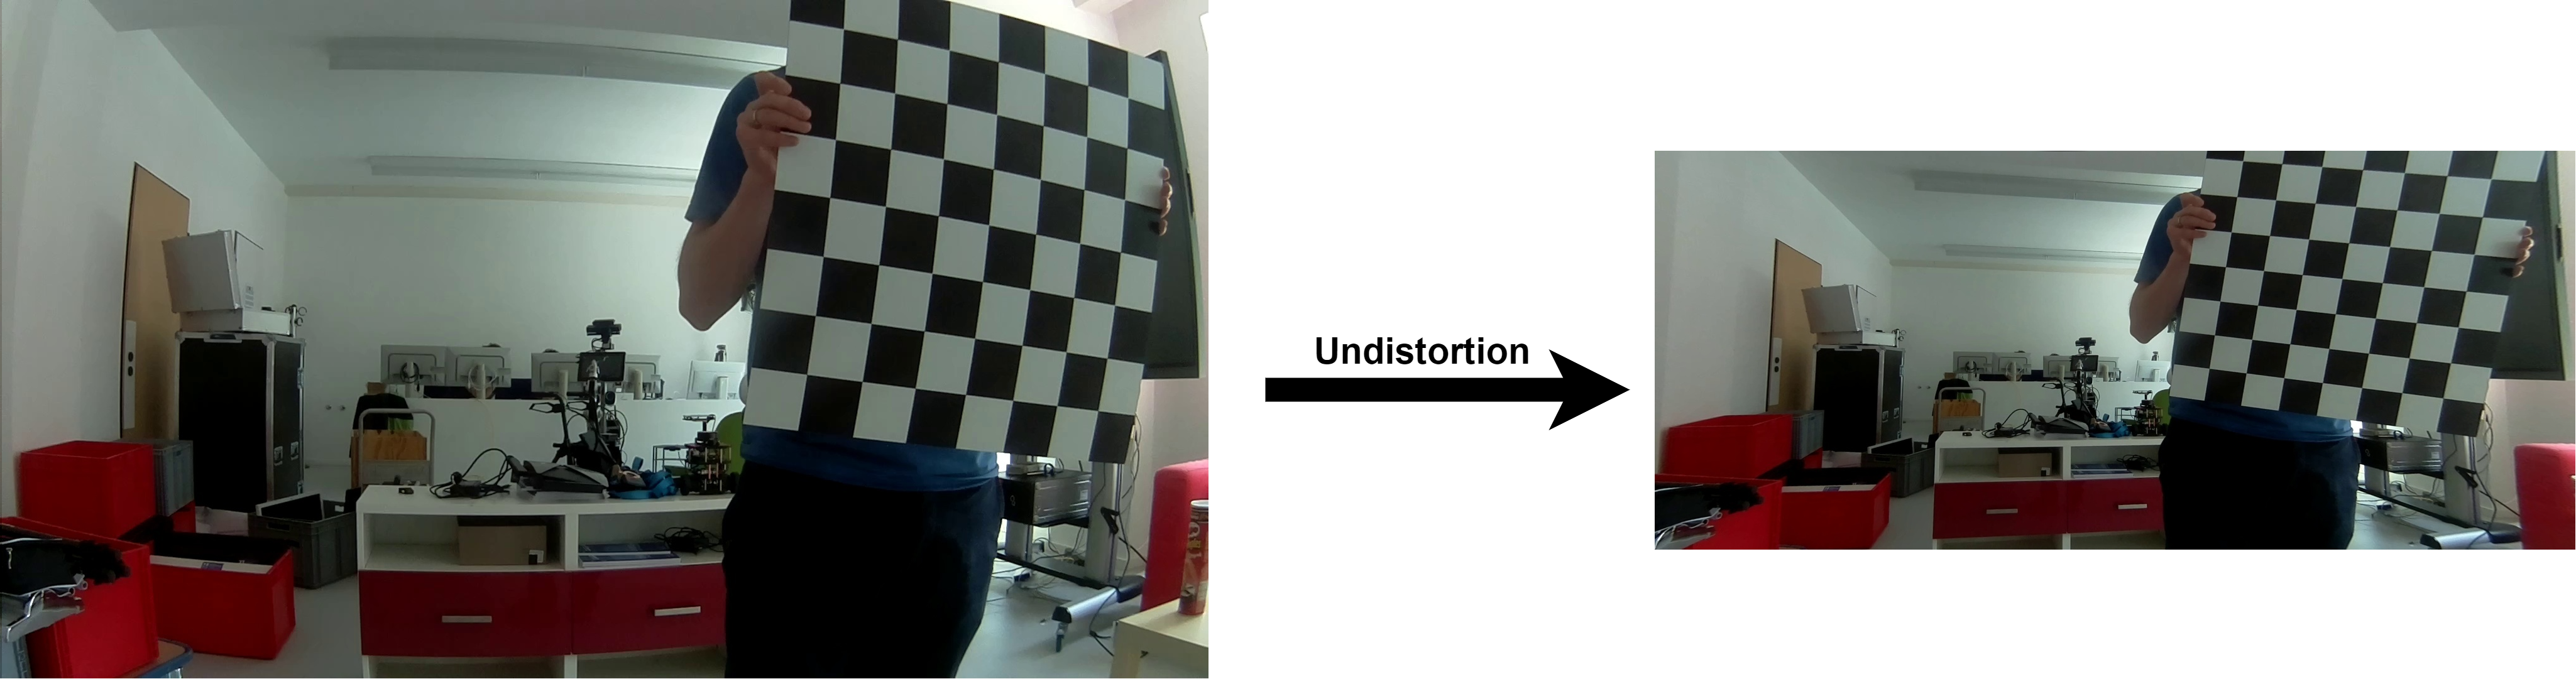
\includegraphics[width=2.5in]{output/res4.png}}
    \caption{Depiction of the final undistortion with the chess board located in the upper right corner.}
    \label{fig:res4}
\end{figure}


% % Here's where you specify the bibliography style file.
% % The full file name for the bibliography style file 
% % used for an ASME paper is asmems4.bst.
% \bibliographystyle{asmems4}
\bibliographystyle{asmems4}

% Here's where you specify the bibliography database file.
% The full file name of the bibliography database for this
% article is asme2e.bib. The name for your database is up
% to you.
\bibliography{asme2e}

\end{document}
